\begin{figure}[t]
    \centering
    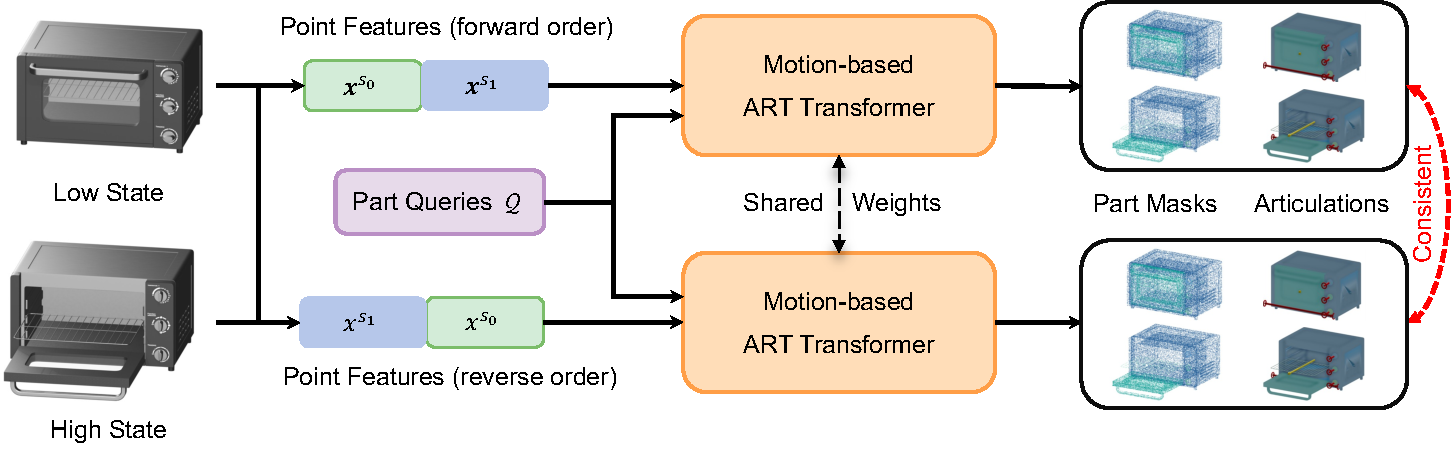
\includegraphics[width=\linewidth]{figs/framework.pdf}
    \caption{\textbf{Overview of \emph{\method}.} Given two observed states of the same object, our framework jointly reasons over cross-state geometry to predict part segmentation and the underlying kinematic structure. We use a set of shared queries to aggregate two-state features, with each query representing a rigid part. The overall Siamese framework consists of two branches: forward order and reverse order. Each branch predicts both part segmentation of two states and articulation parameters.}
    \label{fig:method_overview}
\end{figure}
